\section{Design and Implementation}
\label{sec:Overview}

PEBIL is designed to instrument ELF executables that run on the Linux/x86 platform.
There are several challenges that must be
addressed by any instrumentation tool in this setting, the largest of which include how to correctly
interpret the information found in the text segment of the application and how to organize the
extra information needed by an instrumentation tool given the constraints of the binary format
and platform.

\subsection{Application Code and Data Discovery}
When compilers explicitly produce a text and data segment for an application,
most default to placing the text segment prior and adjacent to the data segment.
However in any ELF executable, data can also be intertwined with code in the text segment of the executable for several reasons, including
the storage of branch target locations (e.g. for a jump table that results from a switch statements) or small data structures 
that provide convenient and efficient look-up of data such as identifiers and descriptors. 
For the sake of correctness of the executable after instrumentation, it is necessary to identify the parts of the text 
section that constitute code and the parts that constitute data. Mishandling of existing data in the text section as code 
may result in instrumented application behavior that differs from the original behavior, especially 
if the instrumentation tool modifies or relocates some part of that data 
to serve the needs of the instrumentation tool. 
Such a change in program behavior may cause outright application failure due to some unintended change in control flow 
or some state condition that is checked by the program.
Alternatively, if code is mistakenly treated as data in the text section, instrumentation might
mistakenly not be inserted into instrumentation code or analysis performed that should be reserved for
application data alone. While this is almost certainly preferable to the situation where data is treated as code, it
is ideal to avoid both situations completely so that the application, 
instrumentation and any resulting analysis is both complete and correct.

PEBIL's code discovery algorithm operates on a per-function basis.
In order to determine which parts of the text sections are functions that are to be subject to its code discovery algorithm, 
PEBIL uses the program's symbol table entries\footnote{The use of the program's symbol table requires that the program be compiled
with debugging information, -g in most cases} to guide it to each function's entry point. The code discovery algorithm then
consists of two possible phases; control-driven disassembly that is backed up by linear disassembly. During the control-driven disassembly phase, 
PEBIL follows the control flow through a function starting at its entry point. If a problem is encountered during disassembly such as 
finding an undefined opcode or an inconsistent control target, 
PEBIL assumes that some part of the disassembly is incorrect and falls back to naive 
disassembly. During the naive disassembly phase, each instruction is disassembled in the order it appears in the
function beginning at the function's entry point. If again a problem 
is found, the function is tagged as uninstrumentable and the disassembly of the function is left incomplete and
hence is ignored for further instrumentation. This 2-phase disassembly algorithm correctly disassembles
an average of 99.8\% of the basic blocks for a set of the SPEC CPU2000 Integer benchmarks.

Problems that can be encountered during both phases of code discovery
are situations where an undefined opcode is encountered, where control jumps to the
middle of an instruction PEBIL has already disassembled, or if control leaves the boundaries of the function via a traditional branch
instruction. In most
cases control-driven disassembly is sufficient to disassemble the entirety of a function, and in most cases control-driven
disassembly is a straightforward process because control either falls through to the following instruction 
or the location of another possible control target is encoded entirely within the instruction itself. But there are also cases
where an indirect address is used by a control instruction, the target residing either at a fixed address (possibly with some offset), in a register, 
or at a location given by a register. The latter two cases are difficult to resolve
without runtime information since the computation of the target address can be arbitrarily complex and can span function
boundaries. Nevertheless, PEBIL performs a peephole examination of the preceding instructions and can determine 
the target address of the branch in most cases.

One of the more common uses of the indirect branch is as part of a jump table. 
Fortunately most compilers use relatively simple calculations to determine targets for jump tables. 
Often an offset is added to a fixed location to determine where the data comprising the branch target
resides. Therefore, such a fixed address found in a nearby instruction 
is treated as the first entry in a table whose remaining entries are considered to be either addresses or offsets.
PEBIL makes an iterative pass over this table to determine the target 
address for each entry in the jump table, stopping when it finds a value in the
table that yields a target address that is outside the function.

\subsection{Instrumentation Code and Data}

Instrumentation generally requires the use of code and data that are not part of the original
executable. In order to insert additional code
and data into an executable, additional space needs to be allocated within the executable in a way that they
will, at load-time, be treated as code and data respectively. Most compilers produce an ELF executable whose
structure is similar to that shown in Figure \ref{fig:Executable}(a). By
convention, most ELF executables use only two loadable segments and indeed some Linux
implementations, such as FreeBSD, only allow two loadable segments. Thus, it is
preferable to incorporate instrumentation text and data into the
existing text and data segments of the application. 

To accommodate the code and data needed for instrumentation, PEBIL prepends the instrumentation code to the existing text
segment\footnote{The amount of space allocated prior to the text section is
controlled by the linker variable \_\_executable\_start. There are cases
where the system does not provide enough space prior to the text segment by
default, in which case PEBIL comes with a set of tools that produces a modified linker
script on the system that provides up to 128MB of space.} and appends the instrumentation data to the
data segment, as shown in Figure \ref{fig:Executable}(b). This
scheme has the added benefit of causing no immediate disturbance to the
addresses of the original data and most of the original text of the program.

\begin{figure}[ht]
\centering
\caption{(a) and (b) show that the
text required by an instrumentation tool is prepended to the application text and the data required by an instrumentation
tool is appended to the data application data.}
\label{fig:Executable}
\subfigure[Layout of an unmodified ELF file.]
{
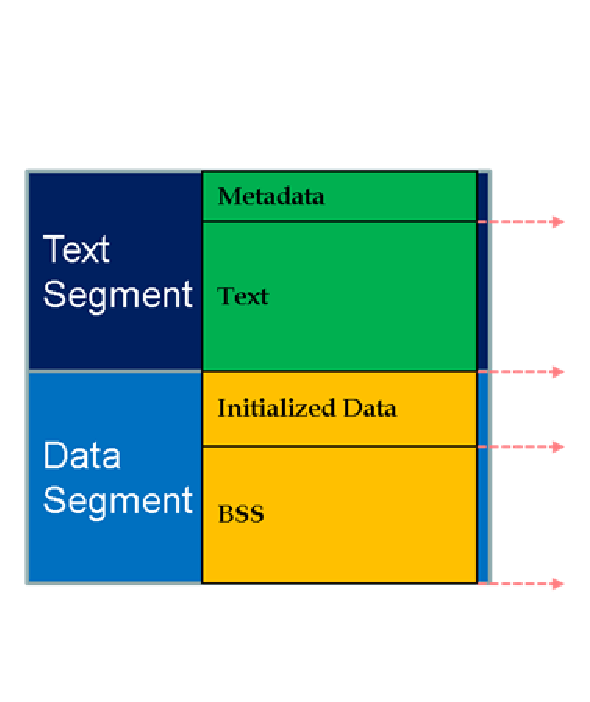
\includegraphics[scale=0.65]{executablep1.eps}
}
\subfigure[Layout of an instrumented ELF file.]
{
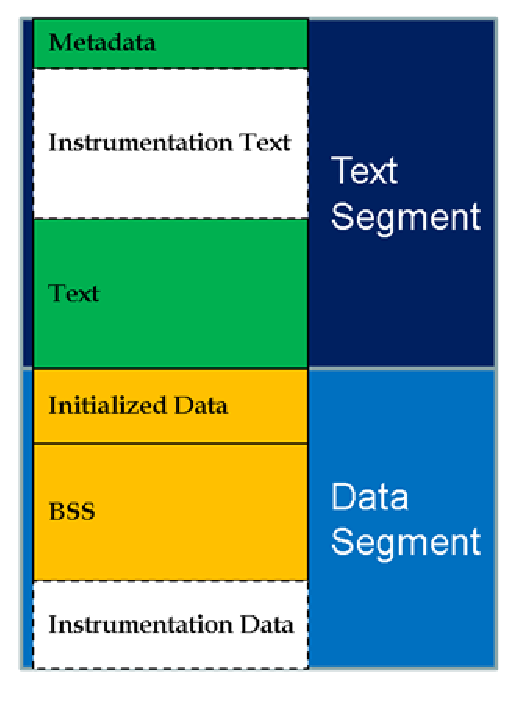
\includegraphics[scale=0.65]{executablep2.eps}
}
\end{figure}

The instrumentation code introduced by PEBIL can be classified by the several distinct functions it
performs. The first
is code that accomplishes the instrumentation tasks as well as any bookkeeping code.
This code sequence, called a \textit{trampoline} \cite{buck2000api}, 
saves any machine state that will be destroyed, performs the instrumentation task, restores
the machine state after the instrumentation, executes the
original instructions that were displaced by the initial control transfer,
and finally restores control to the original code. 
When control is transferred from the application to the
instrumentation code, it is necessary to maintain the machine state of
the application to preserve its original behavior. This machine state
can contain anything modified by the instrumentation code, but in practice is
usually limited to a relatively limited set of registers but in some cases includes
some information about the call stack. 
Since a jump instruction is used at the instrumentation point, the
instrumentation code lacks any information about where control was transferred from. Hence
each instrumentation point uses its own trampoline so that the location of the
instrumentation point can be encoded into an unconditional branch instruction
at the end of the trampoline so that control is returned to the application correctly.

Since some instrumentation tools may need additional data to support the inserted instrumentation code,
PEBIL provides mechanisms to insert and initialize additional data within the executable.
The instrumentation text includes code to, at the beginning of the instrumented 
application run, initialize this additional data for use by the
instrumentation tool. Recall from Figure \ref{fig:Executable} that the instrumentation
data was appended to the end of the application's data segment, after the
application's uninitialized data section (BSS section) in order to preserve the application's 
original addresses. The initialized data and BSS
sections of the data segment are usually implemented in an ELF executable by declaring the size of
the data segment in the executable to be smaller than the size of the data
segment in memory. 

According to the ELF specification \cite{standard1995executable}, the extra part of any
segment whose memory size is greater than its file size should be filled with
zeros by the loader. Hence most programs simply increase the size of the data
segment in memory by the size of the BSS section in order to get an
area that is filled with zeroed, which is reserved for uninitialized data. Since the area following the BSS section is well-suited for
storing additional data for the instrumentation tool, either the entire data
segment's contents, including the applications BSS section and the instrumentation data,
must be included in the executable file or space can be implicitly reserved and later initialized using the
technique currently employed in most ELF files.
Since the BSS section of an application can be very large and explicit inclusion of its contents
into the executable would bloat the size of the executable file unnecessarily, PEBIL uses the implicit
technique to reserve this section for instrumentation data. Therefore the instrumentation data is
temporarily stored with the instrumentation text in the
executable. This data is then copied to the correct location in the data segment once execution
of the instrumented executable begins, thus code to accomplish this is included in the
instrumentation text as well.
